\chapter{Conclusion\label{cha:chapter7}}

 \begin{figure}[h]
 	\centering
 	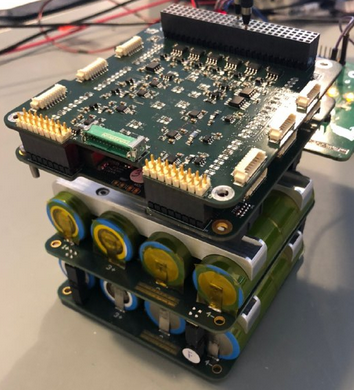
\includegraphics[scale=0.6]{EPS!.png}
 	\caption{EPS assembly (PDU, PPU, Battery board)}
 	\label{fig: EPS!}
 \end{figure}

This master thesis describes the development of the Power Distribution Unit that is designed in combination with Power Processing Unit and Battery Pack board to supply a 6U satellite with  continuous power.\\  


Massive work was made to accomplish all requirements and develop the PDU.
 

 One of the biggest challenges during the PDU design was the switch selection, and their placement on the PCB layout, taking into account the amount of components on the layout and the power channels requirements such as needed voltage, current, the trace width, size and ability to determine an over-current. Another big challenge was the layout structure of the PDU. Due the fact that the PDU should not only be the distribution board for one Descartes Mission, but an universal distribution unit. 
 
  During the tests, the PDU had some issues with a voltage drop on the Hispico line while initiation of the S-band transceiver. The voltage drop occurred due to the high inrush current of the Hispico transceiver. However, after adding an extra capacitors on the output of the switch, voltage drop was reduced and results were satisfactory.    \\ 

First, the PDU was tested using microcontroller Nucleo STM32L073Rz with PSU as a power source and with an electrical load to simulate the load. 

After successful results with Nucleo, PSU and electrical load, the PDU was tested using the flight hardware such as PPU, which included a microcontroller to control the switches and receive data from current sensors, a battery board that provided power for the PDU, and payloads. 
\\ \\
The Power Distribution Board was designed by using Altium Designer and fabricated by Würth Electronics GmbH. All components were soldered by hands and tested according to the test procedure, described in the chapter \ref{6}. Most of the used components have a flight heritage from previous missions, which makes the PDU more promising for the upcoming projects.  \\ 
Power Distribution Unit fits comfortably withing the mechanical structure of the 6U satellite, all the connectors are easily accessible. The
PDU was developed following the standardized design which includes the board dimensions (90.16x95.9mm) and PC104 connector location.
Due to the standardized design, it allows the PDU to be implemented for a 1U, 2U and 3U satellites. \\ \\
Although the PDU was developed and successfully tested for a Descartes Mission, there is still room for future contributions and improvements. The first possible improvement would be a placement of a zero ohm resistor in the parallel to the isolator. This improvement will give an opportunity to choose if isolator is needed. The reason for this improvement occurred while the temperature sensors test connected to the K11. Initially K11 connector was designed for a payload. According to the functional requirements FR4, the PDU shall have isolation for every payload node. However, for a Descartes mission K11 connector was used for a thermal sensors which are part of the satellite bus and have their own isolation.

 Although TPS203x switches have a flight heritage, relatively simple and robust, they are bulky and can not be adjusted for a current limit by changing resistance value, which is a sensitive disadvantage that might be changed in the future versions.  \\ \\
In conclusion, Power Distribution Board was successfully designed,  manufactured and tested according to all requirements. At the moment the flight version of the PDU is ready to fly. 
